\documentclass[12pt, fleqn]{extarticle}

%%===========================================================================================
%%=============================== PACKAGES ==================================================
%%===========================================================================================
\usepackage{blindtext}

\usepackage{array, multirow, tabularx}

\usepackage{color}
\usepackage{xcolor}
\renewcommand{\labelenumii}{{\footnotesize \textbf{\arabic{enumi}.\arabic{enumii}}} }


\usepackage[francais]{babel}
\usepackage[T1]{fontenc}
\usepackage[utf8]{inputenc}
\usepackage{graphicx}



\usepackage{algorithm}
\usepackage[noend]{algpseudocode}
\makeatletter
\def\BState{\State\hskip-\ALG@thistlm}
\makeatother


\usepackage{blkarray}

\usepackage{bm}
\usepackage{hyperref}
\hypersetup{colorlinks=true}


\usepackage{pgf, tikz}
\usetikzlibrary{automata,positioning}
\usetikzlibrary{shapes.multipart}

\usepackage[framemethod=tikz]{mdframed}
\usepackage{showexpl}


\usepackage{verbatim}
\usepackage{fancyvrb}

\usepackage{textcomp}

\usepackage{float, subcaption}
\usepackage[margin=8mm]{caption}
\renewcommand{\captionfont}{\small}
\setlength{\abovecaptionskip}{1pt}

\usepackage{amsmath, amssymb, mathrsfs, mathtools}

\usepackage[final]{pdfpages} 

\renewenvironment{abstract}{%
\hfill\begin{minipage}{0.95\textwidth}
\rule{\textwidth}{1pt}}
{\par\noindent\rule{\textwidth}{1pt}\end{minipage}}

\renewcommand\appendix{\par
  \setcounter{section}{0}
  \setcounter{subsection}{0}
  \setcounter{figure}{0}
  \setcounter{table}{0}
  \renewcommand\thesection{Annexe \Alph{section}}
  \renewcommand\thefigure{\Alph{section}\arabic{figure}}
  \renewcommand\thetable{\Alph{section}\arabic{table}}
}

\usepackage{listings}
\lstset{showstringspaces=false,breaklines=true,breakatwhitespace=true,basicstyle=\scriptsize\ttfamily,numbers=left, numberstyle=\tiny\ttfamily\color{gray}, numbersep=10pt, captionpos=b} 

\usepackage{textcomp}

\usepackage{enumitem}
\renewcommand{\theenumi}{{\scriptsize \textbf{\emph{\arabic{enumi}}}}}

% à activer avec la commande latex2html
%\usepackage{html}

%%===========================================================================================
\usepackage{eso-pic}

\makeatletter
\newlength\@tempdim@x
\newlength\@tempdim@y
% structure des commandes :
%   #1 = deplacement selon x
%   #2 = deplacement selon y
%   #3 = texte à mettre
\newcommand\AtLowerLeftCorner[3]{%
\begingroup
\@tempdim@x=0cm
\@tempdim@y=0cm
\advance\@tempdim@x#1
\advance\@tempdim@y#2
\put(\LenToUnit{\@tempdim@x},\LenToUnit{\@tempdim@y}){\textbf{\textcolor{gray!80}{#3}}}%
\endgroup
}
\newcommand\AtLowerRightCorner[3]{%
\begingroup
\@tempdim@x=\paperwidth
\@tempdim@y=0cm
\advance\@tempdim@x-#1
\advance\@tempdim@y#2
\put(\LenToUnit{\@tempdim@x},\LenToUnit{\@tempdim@y}){\textbf{\textcolor{gray!80}{#3}}}%
\endgroup
}
% ajout de texte ou d'images en haut à gauche, en haut à droite, etc.
%\AddToShipoutPicture{%
%\AtLowerLeftCorner{4cm}{5.5cm}{\rotatebox{90} {\scriptsize LABORATORY UNDER CONSTRUCTION \raisebox{0.1ex}{--} THE CONTENT SHOULD BE TREATED WITH CAUTION}}
%}
\makeatother

\usepackage[left,modulo]{lineno}
%\linenumbers

\usepackage{scrextend}
%%===========================================================================================
%%===========================================================================================
%%===================================== TITLE ================================================
%%===========================================================================================

%pas d'indice dans la bibliographie
\makeatletter
\renewcommand{\@biblabel}[1]{}
\makeatother

\title{%
    \begin{minipage}\linewidth
%    \begin{center}
%        \bfseries\sffamily
%  %       {\huge Les rythmes du gwoka}\\
%    %     \vskip40pt
%      %   {\normalsize -- -- --}
%         \end{center}
         \begin{flushleft}
   %   \vskip20pt
         \bfseries\sffamily
                 \large Les rythmes du gwoka
        \hrulefill
        \end{flushleft}
    \end{minipage}
}

\author{Yann Ics\\ 
%{\small  Anarchic Musical Research Laboratory\\ \& Philosophy of Knowledge\\
{\small %Laboratoire Anarchique\\ de Recherche Musicale \\% \& Philosophie du Savoir\\ et de la Connaissance\\
\href{https://yannics.github.io}{\texttt{https://yannics.github.io}}\\
}
}
\date{
 \begin{minipage}\linewidth
    \begin{center}
    2012 -- 2015
\end{center}
    \end{minipage}
}

%\setlength{\oddsidemargin}{10pt} % Marge gauche sur pages impaires
%\setlength{\evensidemargin}{10pt} % Marge gauche sur pages paires
%\setlength{\marginparwidth}{84pt} % Largeur de note dans la marge
%\setlength{\textwidth}{381pt} % Largeur de la zone de texte (17cm)

\makeatletter
\renewcommand\@maketitle{%
\hfill
\begin{minipage}{0.95\textwidth}
\begin{flushright}
\vskip 2em
\let\footnote\thanks 
{\LARGE \@title \par }
\vskip 2em
{\large \@author \par}
\end{flushright}
\end{minipage}
\vskip 3em \par
}
\makeatother

%%===========================================================================================
%%======================================== BEGIN DOC =========================================
%%===========================================================================================

\begin{document}
  \maketitle
       
  
%\hrulefill

%\vspace*{60pt}


 \thispagestyle{empty}

\hrulefill

\vspace*{10pt}

\begin{center}
    \texttt{[ 2012 -- 2015 ]}
\end{center}

\vspace*{25pt}

%\begin{figure}[h]
%	\begin{center}
%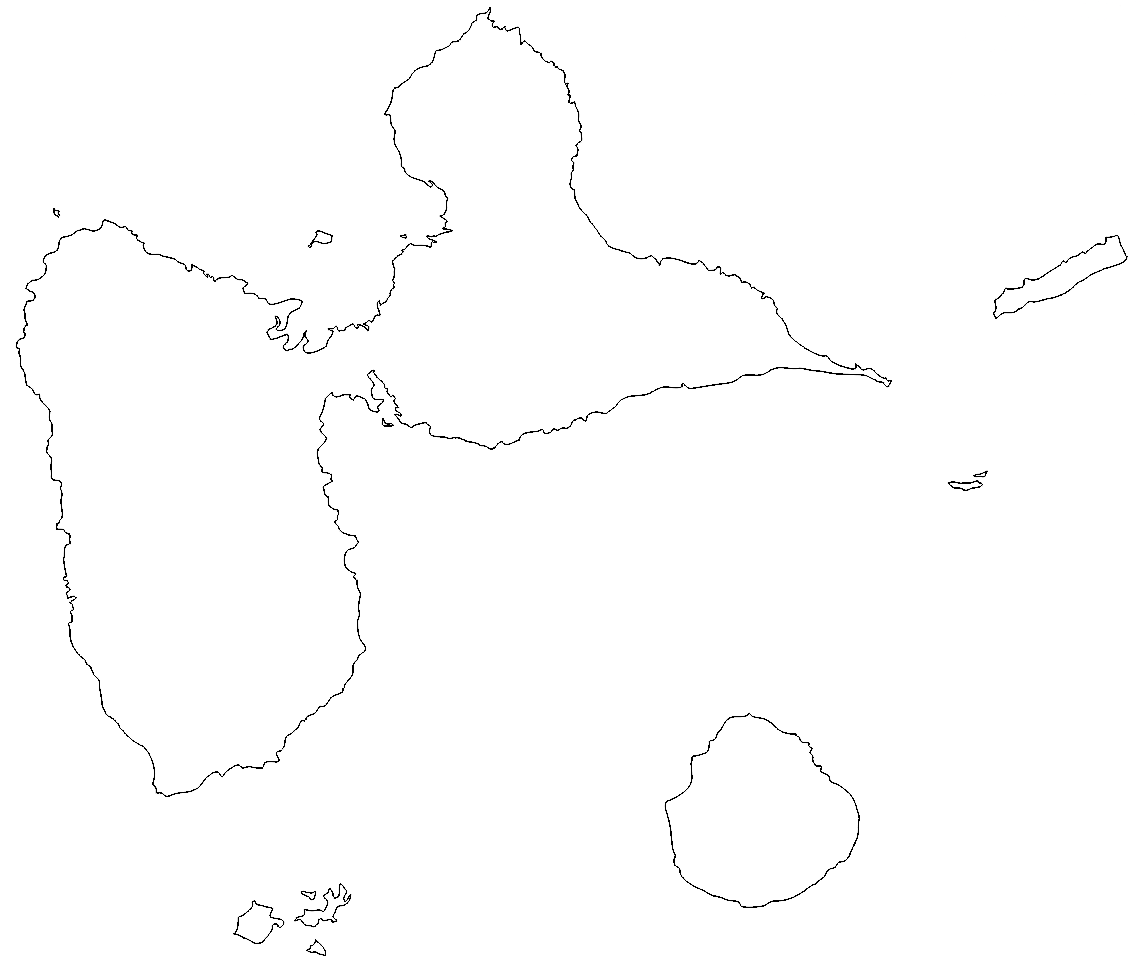
\includegraphics[scale=0.25]{img/gwad.png}
%	\end{center}
%\label{ka}
%\end{figure}
\begin{figure}[h]
	\begin{center}
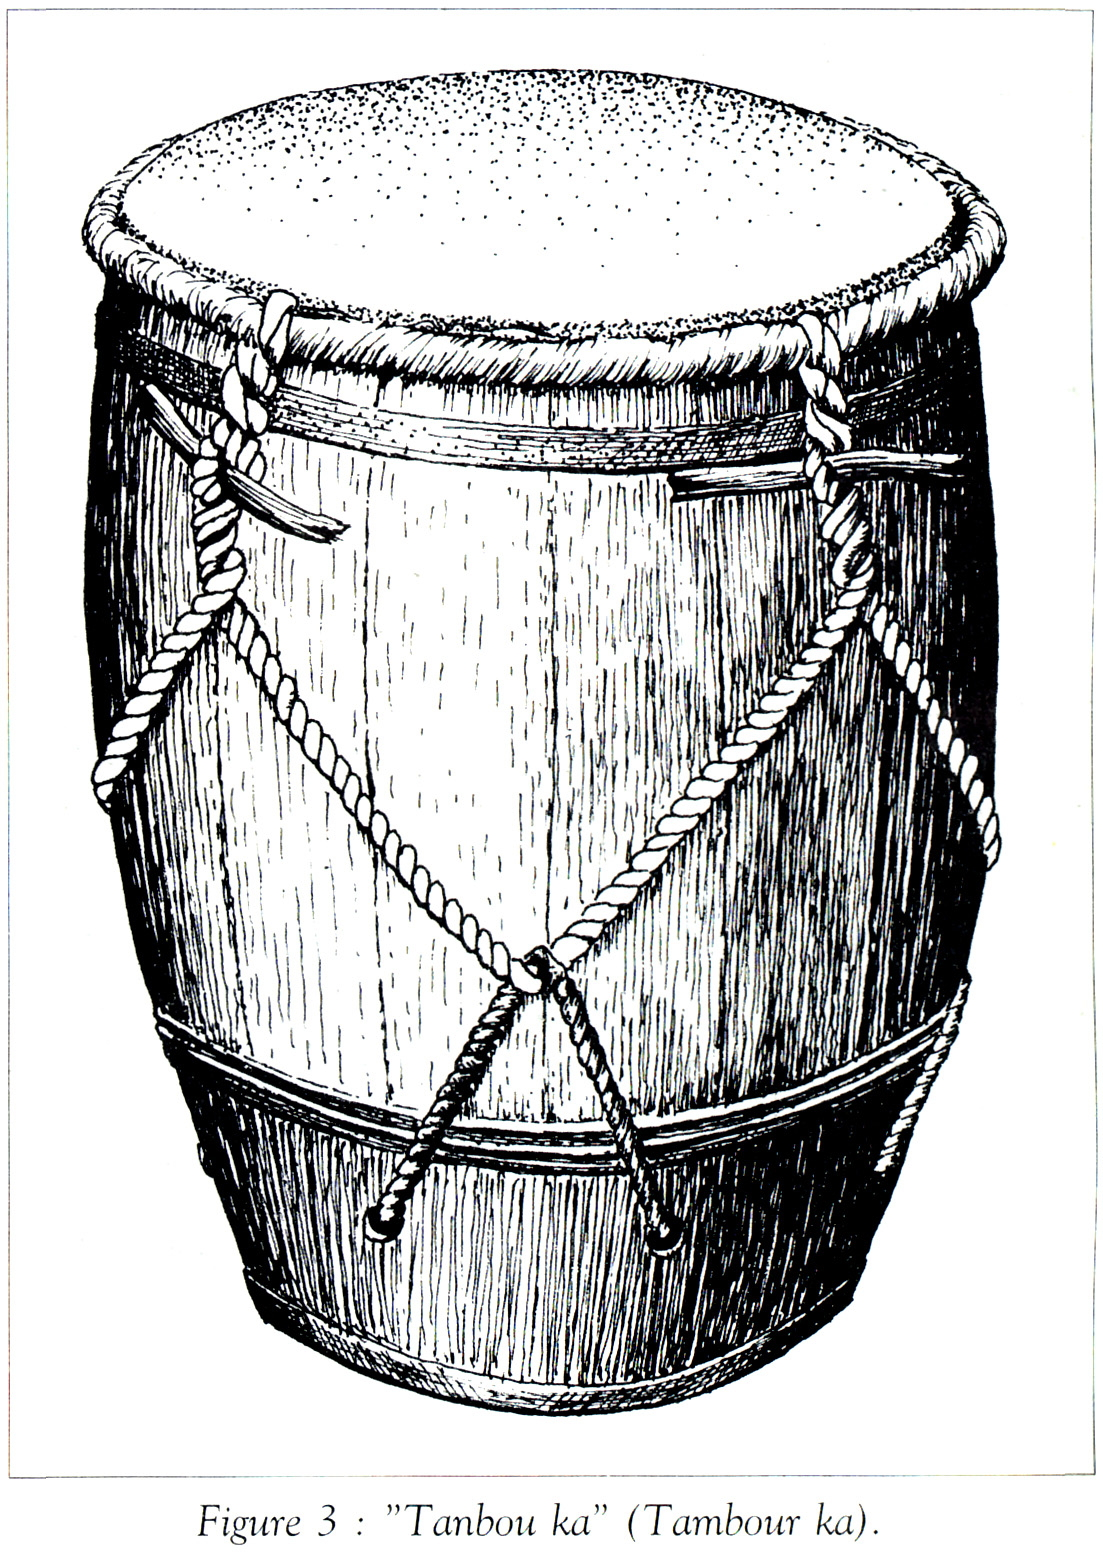
\includegraphics[scale=0.6]{img/ka.jpg}
	\end{center}
\caption{Dessin: Jean-Michel Lisima\protect\footnotemark}
\label{ka}
\end{figure}

\footnotetext{Jean-Michel \textsc{Lisima}, \textit{Fabrication artisanale des tambours}, Absalon, 1993.}



%%===========================================================================================
\clearpage
%\noindent {\large\textbf{Quelques définitions liminaires ...}}

\clearpage
{\noindent {\textsf{\Large \textbf{Le gwoka}}}}
\bigskip
\par
Le Gwoka signifie littéralement « gros tambour » (voir figure~\ref{ka}). Il est la manifestation musicale guadeloupéenne héritée de la musique multi-ethnique des esclaves des anciennes plantations. Chaque rythme -- syncrétisme caraibo-indo-inter-ethno-africain\footnote{Même si à l'origine, le gwoka est manifestement un mélange constitué principalement d'apport ethno-rythmique d'Afrique de l'ouest, le processus de créolisation musical fut aussi diachronique.\\ \indent Certains interprétes de gwoka iront jusqu'à le « jazzifier » -- \textit{cf.} Guy \textsc{Konkèt} (1950-2012), chanteur et tambourinier guadeloupéen;\\ « \textit{Guy Konkèt compte par sa personnalité, par le rôle qu'il a donné au gwoka, le tambour archaïque dont il fait la gloire présente, et par sa méthode. Liant à la fois tradition et modernité, ouvrant la '}musique de vieux nègres\textit{' à tous les avenirs, faisant le lien entre les musiques autochtones et le jazz le plus free, ouvrant sa voix à tous les possibles, excédant largement les limites gracieuses des supposées 'musiques du monde'. Sans rien masquer de ses combats politiques et sociaux.} » [ Décés de Guy Konkèt, musicien guadeloupéen, l'âme du gwoka, Francis \textsc{Marmande}, \textit{Le Monde} 30 mai 2012 ].\label{ftn:konk}} -- est associée à une activité spécifique et se compte à la base au nombre de sept: le Léwoz, le Padjanbèl, le Graj, le Woulé, le Kaladja, le Toumblak et le Menndé\footnote{L'orthographe de ces rythmes peut varier selon qu'elle soit créole ou bien ethnographique.}. 

%\bigskip
\bigskip

\bigskip

\par
Le gwoka s'inscrit dans une performance où interviennent trois acteurs différents. Le premier est le chanteur -- accompagné d'un choeur -- exprimant un chant de type responsorial; le second est le marqueur -- à la percussion soliste -- soutenu par les boulas (exécutant un des rythmes de base initié ou soutenu par le marqueur); le troisième acteur est le danseur. Chaque acteur -- ou soliste -- contribue à la dynamique de l'ensemble selon des codes intrinsèques à l'expression musicale du gwoka à un moment donné (dépendant de la personnalité des acteurs, du contexte social, du prétexte de la performance, ... ). La part d'improvisation reste la règle, laquelle part peut être comparée à la manière dont les musiciens de jazz la pratiquent. 

\bigskip
\par
La partie instrumentale est composée de deux types de tambours: l'un dans le registre grave est appelé \textit{boula} avec lequel on frappe l'un des rythmes de base, l'autre plus aigu est appelé \textit{makè} destiné à l'improvisation du marqueur.

%\bigskip

\bigskip
\bigskip
\small
\clearpage
{\noindent {\textsf{\Large \textbf{Les 7 rythmes de base}}}}
\bigskip
\bigskip
 
%%%%%%%%%%%%%%%%%%%%%%%%%%%%%%%%%%%%%%%%%%%%%%%%%%
%         	LÉWOZ
%%%%%%%%%%%%%%%%%%%%%%%%%%%%%%%%%%%%%%%%%%%%%%%%%%

{\large \textbf{Léwoz}}

Rythme de référence du gwoka, il exprime la lutte.
Il existe deux façons d'exécuter le léwoz selon la région -- à savoir le léwoz de Grande-Terre et le \textit{léwoz in-dès-twas} (de Sainte-Rose).
\bigskip
\begin{quote}
{%
\parindent 0pt
\noindent
\ifx\preLilyPondExample \undefined
\else
  \expandafter\preLilyPondExample
\fi
\def\lilypondbook{}%
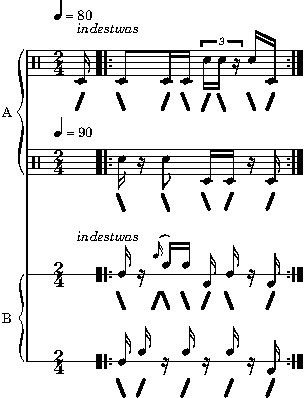
\includegraphics{87/lily-2de452d3-1}%
% eof

\ifx\postLilyPondExample \undefined
\else
  \expandafter\postLilyPondExample
\fi
}
\end{quote}


%%%%%%%%%%%%%%%%%%%%%%%%%%%%%%%%%%%%%%%%%%%%%%%%%%
%			PADJAMBEL
%%%%%%%%%%%%%%%%%%%%%%%%%%%%%%%%%%%%%%%%%%%%%%%%%%

\bigskip
\bigskip
{\large \textbf{Padjambel}}

Rythme de caractère guerrier au sens d'affranchissement à tout ce qui est avilissant.
\bigskip
\begin{quote}
{%
\parindent 0pt
\noindent
\ifx\preLilyPondExample \undefined
\else
  \expandafter\preLilyPondExample
\fi
\def\lilypondbook{}%
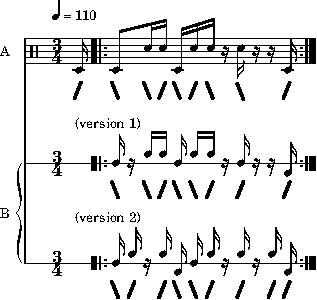
\includegraphics{82/lily-6d9f6c8a-1}%
% eof

\ifx\postLilyPondExample \undefined
\else
  \expandafter\postLilyPondExample
\fi
}
\end{quote}

%%%%%%%%%%%%%%%%%%%%%%%%%%%%%%%%%%%%%%%%%%%%%%%%%%
%			GRAJ
%%%%%%%%%%%%%%%%%%%%%%%%%%%%%%%%%%%%%%%%%%%%%%%%%%
\clearpage
\bigskip
\bigskip
{\large \textbf{Graj}}

Rythme de travail des champs.
\bigskip
\begin{quote}
{%
\parindent 0pt
\noindent
\ifx\preLilyPondExample \undefined
\else
  \expandafter\preLilyPondExample
\fi
\def\lilypondbook{}%
\includegraphics{4c/lily-56731605-1}%
% eof

\ifx\postLilyPondExample \undefined
\else
  \expandafter\postLilyPondExample
\fi
}
\end{quote}


%%%%%%%%%%%%%%%%%%%%%%%%%%%%%%%%%%%%%%%%%%%%%%%%%%
%			WOULÉ
%%%%%%%%%%%%%%%%%%%%%%%%%%%%%%%%%%%%%%%%%%%%%%%%%%
%\clearpage

\bigskip
\bigskip
{\large \textbf{Woulé}}

Rythme de travail.
\bigskip
\begin{quote}
{%
\parindent 0pt
\noindent
\ifx\preLilyPondExample \undefined
\else
  \expandafter\preLilyPondExample
\fi
\def\lilypondbook{}%
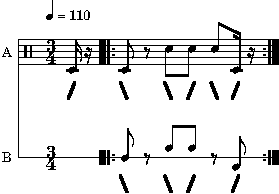
\includegraphics{89/lily-1a2b1a45-1}%
% eof

\ifx\postLilyPondExample \undefined
\else
  \expandafter\postLilyPondExample
\fi
}
\end{quote}

%%%%%%%%%%%%%%%%%%%%%%%%%%%%%%%%%%%%%%%%%%%%%%%%%%
%			KALADJA
%%%%%%%%%%%%%%%%%%%%%%%%%%%%%%%%%%%%%%%%%%%%%%%%%%
%\clearpage
\bigskip
\bigskip

{\large \textbf{Kaladja}}

Se joue lentement -- dans ce cas, ce rythme exprime la souffrance ou la peine -- ou rapidement à l'instar du Toumblack.
\bigskip
\begin{quote}
{%
\parindent 0pt
\noindent
\ifx\preLilyPondExample \undefined
\else
  \expandafter\preLilyPondExample
\fi
\def\lilypondbook{}%
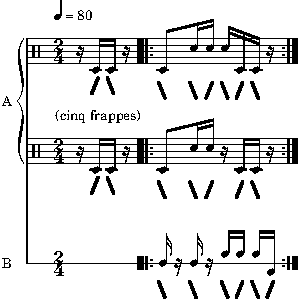
\includegraphics{a2/lily-64356649-1}%
% eof

\ifx\postLilyPondExample \undefined
\else
  \expandafter\postLilyPondExample
\fi
}
\end{quote}

%%%%%%%%%%%%%%%%%%%%%%%%%%%%%%%%%%%%%%%%%%%%%%%%%%
%			TOUMBLACK
%%%%%%%%%%%%%%%%%%%%%%%%%%%%%%%%%%%%%%%%%%%%%%%%%%
\bigskip
\bigskip
{\large \textbf{Toumblack}}

Rythme de fête dédié à la danse. Une partie du toumblack -- appelé \textit{tumblak chiré} -- consiste à accélérer le tempo jusqu'à l'ivresse, et se termine ainsi par une coda.
\bigskip
\begin{quote}
{%
\parindent 0pt
\noindent
\ifx\preLilyPondExample \undefined
\else
  \expandafter\preLilyPondExample
\fi
\def\lilypondbook{}%
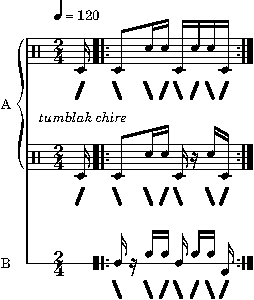
\includegraphics{7a/lily-a9c4e824-1}%
% eof

\ifx\postLilyPondExample \undefined
\else
  \expandafter\postLilyPondExample
\fi
}
\end{quote}


%%%%%%%%%%%%%%%%%%%%%%%%%%%%%%%%%%%%%%%%%%%%%%%%%%
%			MENDÈ
%%%%%%%%%%%%%%%%%%%%%%%%%%%%%%%%%%%%%%%%%%%%%%%%%%
%\clearpage

\bigskip
\bigskip
{\large \textbf{Mendè}}

Rythme de fête à caractère licencieux.
\bigskip
\begin{quote}
{%
\parindent 0pt
\noindent
\ifx\preLilyPondExample \undefined
\else
  \expandafter\preLilyPondExample
\fi
\def\lilypondbook{}%
\includegraphics{ad/lily-697ca8fb-1}%
% eof

\ifx\postLilyPondExample \undefined
\else
  \expandafter\postLilyPondExample
\fi
}
\end{quote}

%%%%%%%%%%%%%%%%%%%%%%%%%%%%%%%%%%%%%%%%%%%%%%%%%%

\bigskip
\bigskip
\par 
A - D'après Jean-Pierre \textsc{Solvet}, \textit{Solfège du tambour ka}. L'Harmattan, Paris 2007. 
\par
B - D'après \href{http://www.lameca.org}{LAMECA} - Médiathéque Caraïbe Dettino Lara, consulté en 2012. \\
%En ligne $\rightarrow$ \href{http://www.lameca.org/dossiers/gwoka/musique/rythmes/rythm.html}{\texttt{\footnotesize http://www.lameca.org/dossiers/gwoka/musique/rythmes/rythm.html}}
\par
* voir note \ref{ftn:konk} page \pageref{ftn:konk}.
%%%%%%%%%%%%%%%%%%%%%%%%%%%%%%%%%%%%%%%%%%%%%%%%%%

 %%===========================================================================================
%%======================================== END DOC ==========================================
%%===========================================================================================

\end{document}